\section{Fallstudie: Gleichstromantrieb}

\subsection{Modellierung}{53}
\begin{center}
    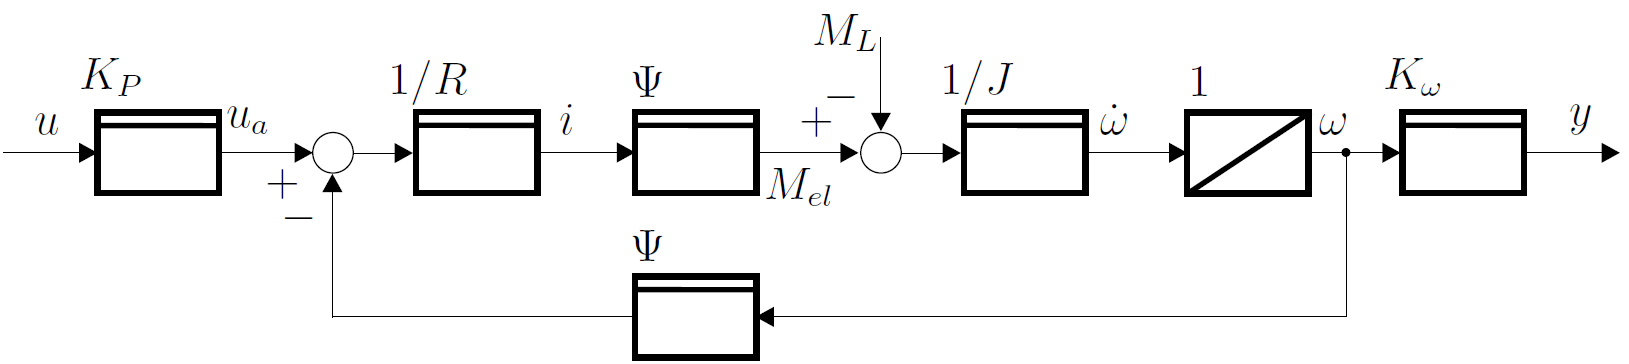
\includegraphics[width=0.75\columnwidth]{images/vereinfachtes_modell_gleichstromantrieb.png} 
\end{center}
Der Gleichstromantrieb kann als $\text{PT}_1$-Glied mit zwei Eingängen $u(t)$ und $M_L(t)$ modelliert werden. $M_L(t)$ entspricht
einer durch Wirbelströme erzeugte \textbf{Störung}.
$$ \boxed{ \underbrace{\frac{R \cdot J}{\Psi^2}}_{T} \dot{y}(t) + y(t) = \underbrace{\frac{K_P \cdot K_{\omega}}{\Psi}}_{K_1} u(t)
    - \underbrace{\frac{R \cdot K_{\omega}}{\Psi^2}}_{K_2} M_L(t) } $$


\subsubsection{Parameter-Identifikation}

\begin{minipage}[c]{0.48\columnwidth}
    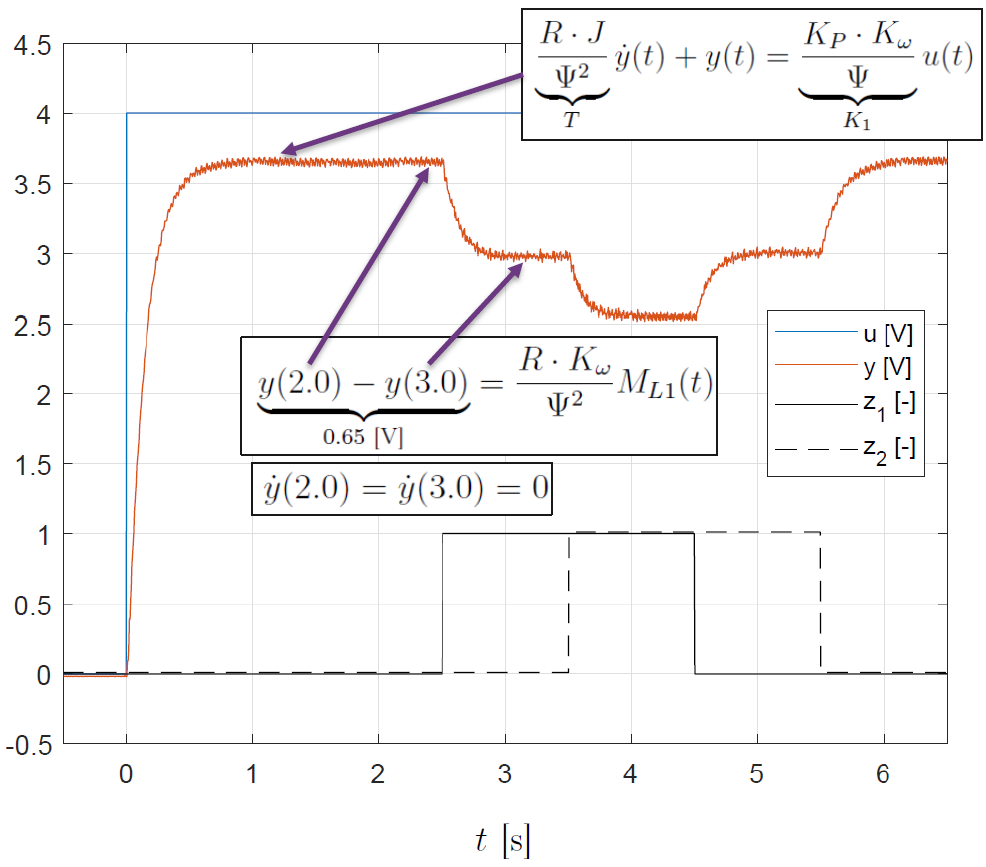
\includegraphics[width=\columnwidth]{images/gleichstrommodell_parameteridentifikation.png}
\end{minipage}
\hfill
\begin{minipage}[c]{0.48\columnwidth}
    Aus der \textbf{Sprungantwort} können einige Parameter abgelesen werden. Einige weitere Parameter sind aus Datenblättern bekannt.
    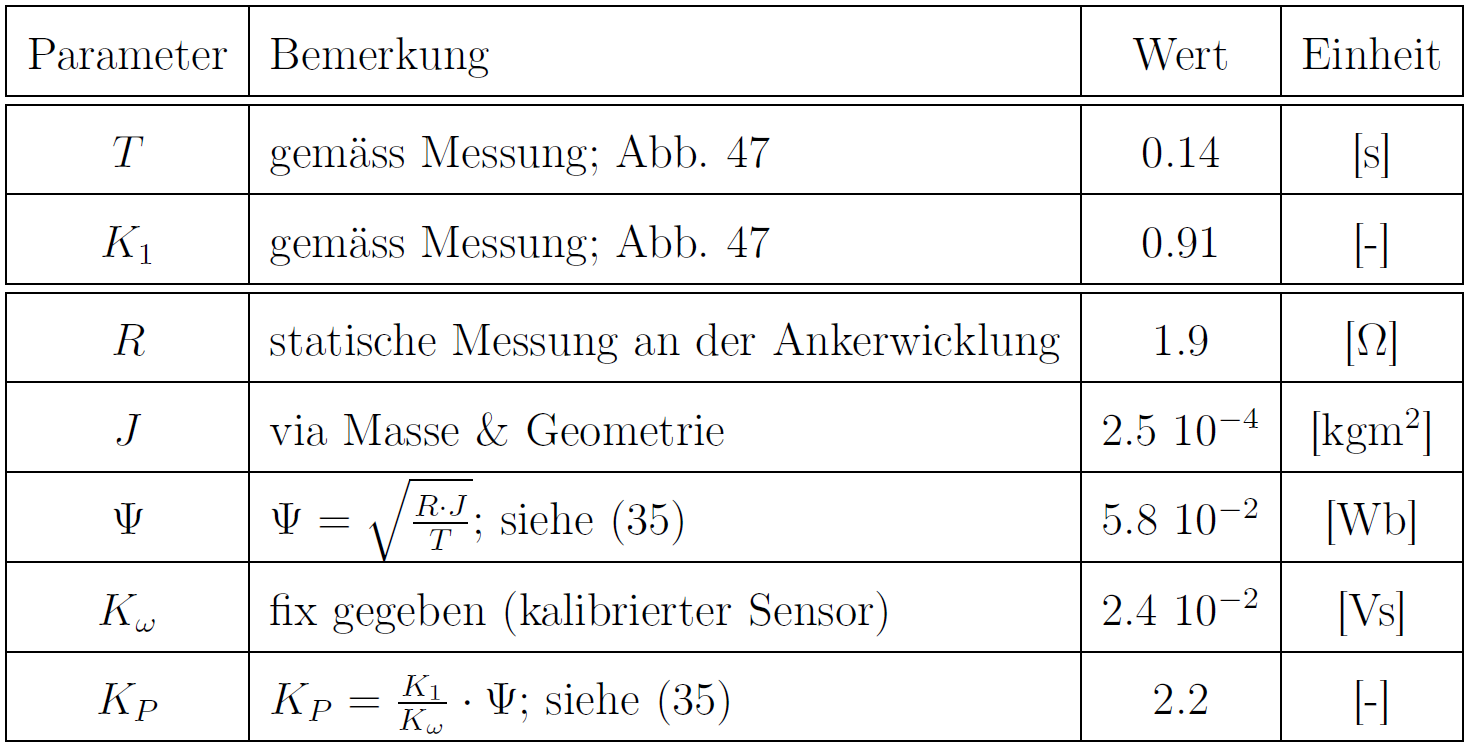
\includegraphics[width=\columnwidth]{images/gleichstrommodell_parameter.png}
    $M_{L1} = 4.8 \cdot 10^{-2} \, [\newton \meter]$
\end{minipage}


\subsection{Gleichstromantrieb mit Steuerung}{148-149}

Die Grösse $\omega$ soll im \textbf{steady-state} gesteuert werden \textrightarrow\ Ableitungen 0, keine Störungen \\
Zu steuern: $\omega = 25 \cdot 2 \pi$, $K_{\omega} \cdot \omega = y = 3.77 \, \volt$ \textrightarrow\ Finde Wert der Eingangsgrösse $u(t)$
$$ \boxed{ \text{Im steady-state: } \xcancel{ \underbrace{\frac{R \cdot J}{\Psi^2}}_{T} \dot{y}(t) } + y_{\rm stat}(t) = \underbrace{\frac{K_P \cdot K_{\omega}}{\Psi}}_{K_1} u(t)
    -  \xcancel{ \underbrace{\frac{R \cdot K_{\omega}}{\Psi^2}}_{K_2} M_L(t) } }$$

$$ y_{\rm stat} = \frac{K_P \cdot K_{\omega}}{\Psi} u_{\rm stat} \qquad  \underrightarrow{y_{\rm stat} = K_{\omega} \cdot \omega } \qquad 
    \omega_{\rm stat} = \frac{K_p}{\Psi} u_{\rm stat}  $$
$$ \text{\textrightarrow\ } u_{\rm stat} = \frac{\Psi}{K_P} \omega_{\rm stat}  = \frac{\Psi}{K_P} 25 \cdot 2 \pi = 4.14 \, \volt \quad  $$


\subsubsection{Probleme der Steuerung}

\begin{minipage}[c]{0.4\columnwidth}
    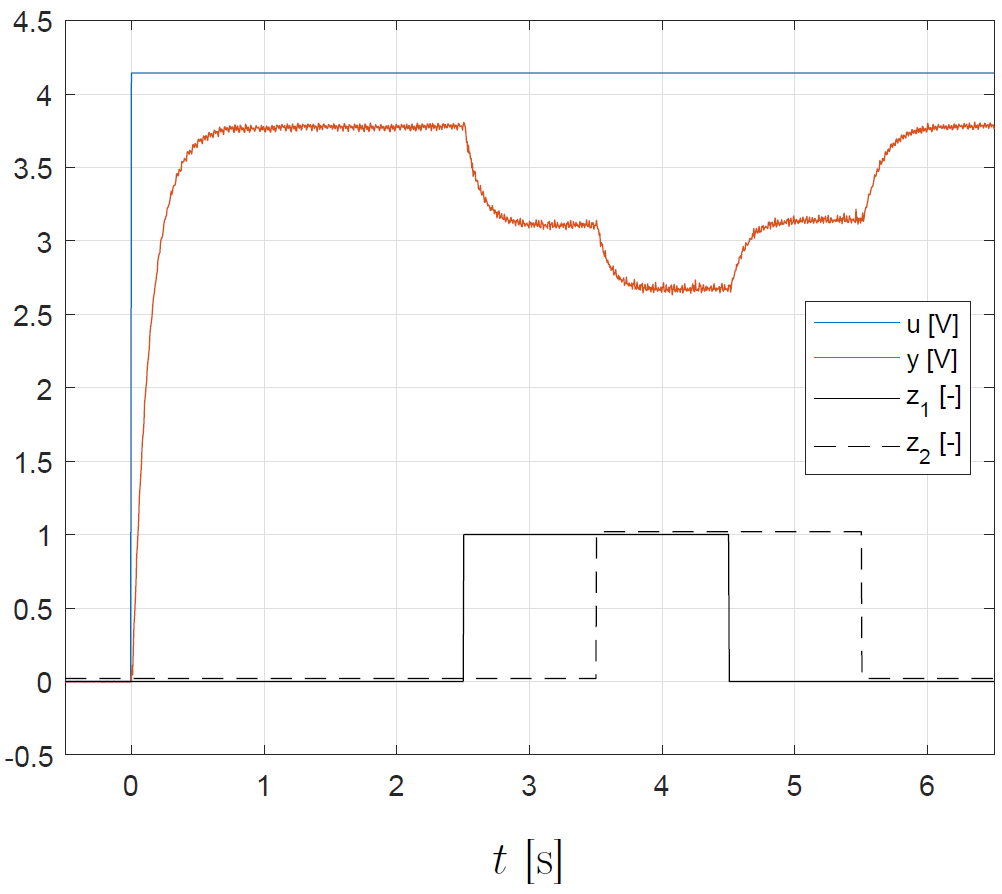
\includegraphics[width=\columnwidth]{images/gleichstromantrieb_steuerung_step-response.png}
\end{minipage}
\hfill
\begin{minipage}[c]{0.48\columnwidth}
    \begin{itemize}
        \item Endwert wird zwar erreicht, aber wenn $K_P$ oder $\Psi$ variieren wird dies nicht mehr der Fall sein
        \item Die Drehzahländerung ist 'langsam' (gemäss Zeitkonstante $T$). (Ein höheres $u$ zu Beginn könnte $T$ verkürzen)
        \item \textbf{Die Steuerung reagiert nicht auf die Störungen!}
    \end{itemize}
\end{minipage}


\subsection{Gleichstromantrieb mit P-Regler}{149-150}
\label{P-Regler}

\begin{minipage}[c]{0.4\columnwidth}
    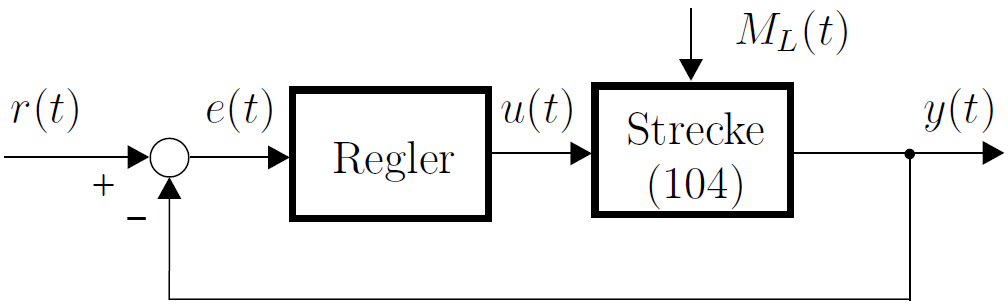
\includegraphics[width=\columnwidth]{images/gleichstromantrieb_p-regler.png}
\end{minipage}
\hfill
\begin{minipage}[c]{0.48\columnwidth}
    $$ u(t) = K_R \cdot e(t) = K_R \cdot ( r(t) - y(t) )$$
\end{minipage}

$$ \boxed{ \text{Geschlossener Regelkreis: } \underbrace{\frac{T}{1 + K_1 K_R}}_{T_f} \dot{y}(t) + y(t) = \underbrace{\frac{K_1 K_R}{1 + K_1 K_R}}_{K_f} r(t)
    - \underbrace{\frac{K_2}{1 + K_1 K_R}}_{K_z} M_L(t) } $$

Damit der Sollwert $r(t)$ erreicht wird (wenn keine Störung $M_L(t)$ vorhanden ist), muss $K_F = 1$ sein
\textrightarrow\ $K_R$ muss sehr gross sein


\subsubsection{Eigenschaften des P-Reglers}

\begin{minipage}[c]{0.4\columnwidth}
    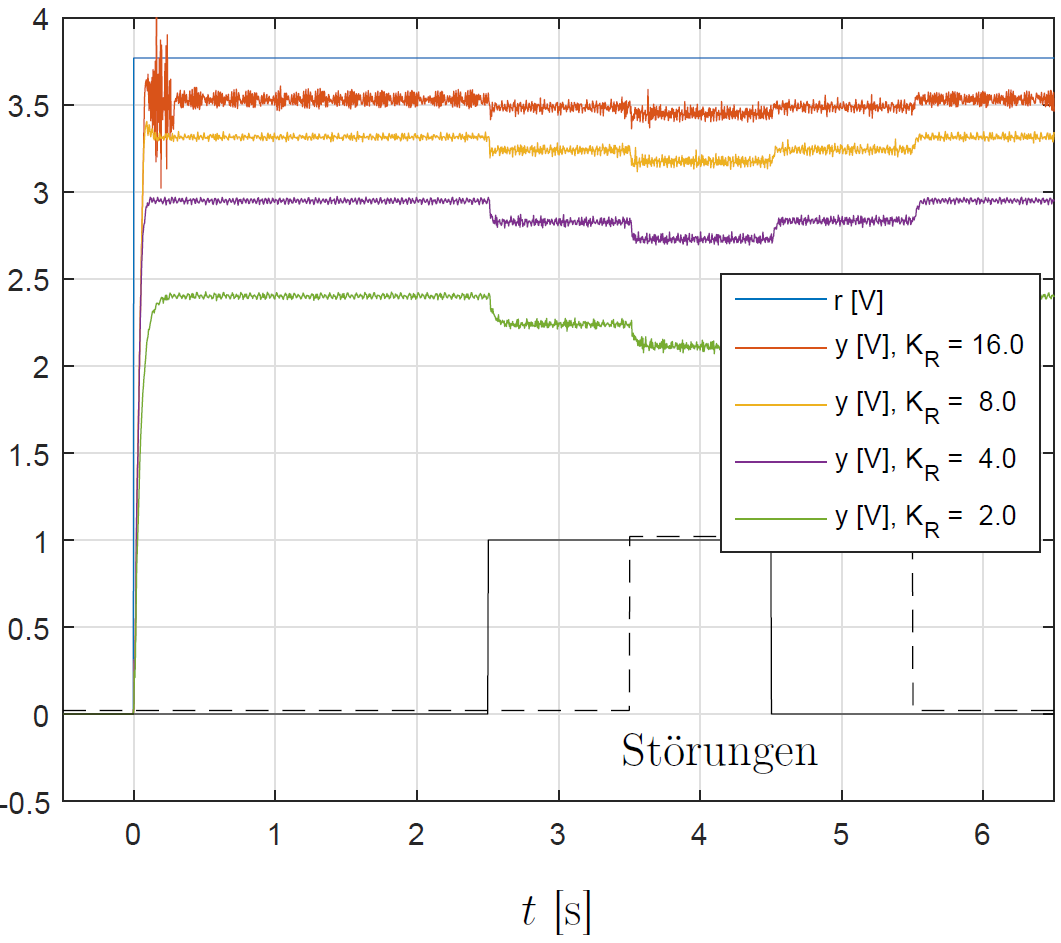
\includegraphics[width=\columnwidth]{images/gleichstromantrieb_p-regler_step-response.png}
\end{minipage}
\hfill
\begin{minipage}[c]{0.58\columnwidth}
    \begin{itemize}
        \item Für $K_R \to \infty$ werden die Zeitkonstante $T_f$ und der Einfluss der Störung $M_L(t)$ beliebig klein \\
            \textrightarrow\ DGL konvergiert zu $y(t) = r(t)$
        \item Für kleine $K_R$ wird Endwert nicht erreicht \\
            \textrightarrow\ statischer Fehler
        \item Stellgrösse $u(t)$ sättigt aufgrund von physikalischen Gegebenheiten \textrightarrow\ Prozess wird \textbf{nichtlinear}
            \textrightarrow\ Überschwinger
        \item Messrauschen wird ebenfalls verstärkt (P-Regler verstärt \textbf{alle} Frequenzen) 
    \end{itemize}
\end{minipage}

\textrightarrow\ \textbf{Es bleibt ein stationärer Fehler!} Dafür reagiert der P-Regler schnell.


\subsection{Gleichstromantrieb mit I-Regler}{151-152}

\begin{minipage}[t]{0.48\columnwidth}
    \begin{center}
        \myul{I-Regler ($K_R$ einstellbar)}
    \end{center}
    $$ u(t) = K_R \int\limits_0^t \underbrace{ r(\tau) - y(\tau)}_{e(\tau)} \, \diff \tau $$
\end{minipage}
\hfill
\begin{minipage}[t]{0.48\columnwidth}
    \begin{center}
        \myul{E-Motor (Strecke, $\text{PT}_1$-System)}
    \end{center}
    $$ T \cdot \dot{y}(t) + y(t) = K_1 \cdot u(t) - K_2 \cdot M_L(t) $$
\end{minipage}

\textrightarrow\ $u(t)$ von I-Regler in Gleichung der Strecke einsetzen, ableiten, umsortieren

$$ \boxed{ \text{PT}_2 \text{-System:} \quad \underbrace{ \frac{T}{K_1 \cdot K_R} }_{T_f^2} \ddot{y}(t) + \underbrace{ \frac{1}{K_1 \cdot K_R} }_{2 \zeta_f T_f} \dot{y}(t) + y(t) 
    = \underbrace{1}_{K_f} r(t) - \frac{K_2}{K_1 \cdot K_R} \dot{M}_L(t) } $$


\subsubsection{Eigenschaften des I-Reglers}

\begin{minipage}[c]{0.48\columnwidth}
    \begin{itemize}
        \item $T_f = \sqrt{ \frac{T}{K_1 \cdot K_R} }$, $\zeta_f = \frac{1}{2 \sqrt{T K_1 K_R}}$
        \item \textbf{Der Integrator sorgt dafür, dass im steady-state kein stationärer Fehler auftritt} ($e(t) = 0$)
        \item Für grosse $K_R$ wird $T_f$ klein, die Sprungantwort schneller (erwünscht)
        \item Für grosse $K_R$ wird $\zeta_f$ klein, die Überhöhung grösser (unerwünscht)
        \item \textrightarrow\ Kompromiss finden
    \end{itemize}
\end{minipage}
\hfill
\begin{minipage}[c]{0.48\columnwidth}
    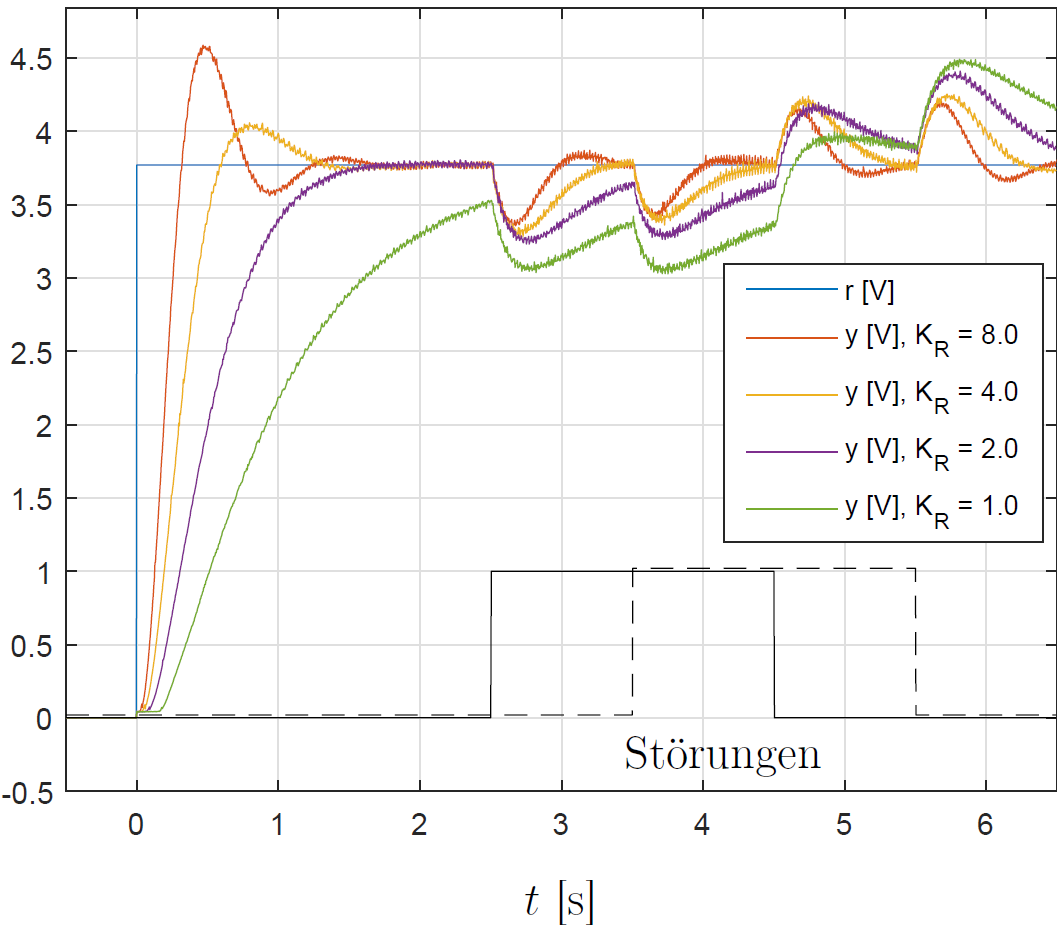
\includegraphics[width=\columnwidth]{images/gleichstromantrieb_i-regler_step_response.png}
\end{minipage}


\subsection{Gleichstromantrieb mit PI-Regler}{152-154}

Vorteile von P-Regler und I-Regler sollen kombiniert werden:
\begin{itemize}
    \item P-Regler für schnelle Reaktion
    \item I-Regler für statische Fehlerunterdrückung
        \textrightarrow\ Parameter $K_R$ und $T_N$ einstellbar
\end{itemize}

\vspace{-0.4cm}
$$ \text{PI-Regler:} \quad u(t) = \frac{1}{T_N} \Big( \int\limits_0^t e(\tau) \, \diff \tau + e(t) \Big) K_R
    \; \laplace \; U(s) = \frac{1}{T_N} \Big( \frac{1}{s} E(s) + E(s) \Big) K_R $$
$$ \text{E-Motor:} \quad T \dot{y}(t) + y(t) = K_1 u(t) - K_2 M_L(t) 
    \; \laplace \; T s Y(s) + Y(s) = K_1 U(s) - \cancel{ K_2 M_L(s)} $$

\vspace{-0.3cm}
\begin{minipage}[t]{0.5\columnwidth}
    $$ \text{UTF Regler: } G_R(s) = \frac{U(s)}{E(s)} = K_R \Big( \frac{1}{T_N} \frac{1}{s} + 1 \Big) $$
\end{minipage}
\hfill
\begin{minipage}[t]{0.46\columnwidth}
    $$ \text{UTF Strecke: } G_S(s) = \frac{Y(s)}{U(s)} = \frac{K_1}{T s + 1} $$
\end{minipage}

Der  Parameter $T_N$ des PI-Reglers wird so gewählt, dass der \textbf{offene Regelkreis} $G_0(s)$ einem \textbf{Integrator} entspricht!
\textrightarrow\ \textbf{Pol-Nullstellenkürzung!}

$$ G_0(s) = G_R(s) \cdot G_S(s) = K_R \frac{1 + T_N s}{T_N s} \cdot \frac{K_1}{T s + 1} \overset{T_N = T}{=} K_R \frac{K_1}{T_N s} $$

Für den \textbf{geschlossenen Regelkreis} ergibt sich somit ein $\text{PT}_1$-System mit Verstärkung $1$\\
(\textrightarrow\ kein statischer Fehler im steady-state). Die Zeitkonstante $T_{\rm geschl}$ wird mit $K_R$ des Reglers eingestellt.

$$ G_f(s) = \frac{G_0(s)}{1 + G_0(s)} =  \frac{\frac{K_R  K_1}{T_N s} }{1 \frac{K_R  K_1}{T_N s}} = \frac{K_R K_1}{T_N s + K_1 K_R} = \frac{1}{\frac{T_N}{K_R  K_1}s + 1} $$


\subsubsection{Pol-Nullstellenkürzung}

Wird durchgeführt, um den \textbf{offenen Regelkreis} zu vereinfachen. Pole und Nullstellen der Strecke werden mit einer geeigneten
Wahl der Parameter des Reglers kompensiert. \\
\textrightarrow\ \textbf{Idealfall: offener Regelkreis verhält sich wie ein Integrator.}

\begin{itemize}
    \item Betrachtung UTF des offenen Regelkreises
    \item Parameter des Reglers so wählen, dass man Polstelle mit einer Nullstelle kürzen kann \\
        \textrightarrow\ Diejenige Polstelle, welche am frühesten 'zündet', ist bevorzugt zu kürzen!
\end{itemize}


\subsubsection{Eigenschaften des PI-Reglers}

\begin{minipage}[c]{0.48\columnwidth}
    \begin{itemize}
        \item Zeitkonstante und Verstärkung unabhängig voneinander einstellbar
        \item Kein Überschwingen
        \item \textbf{Konstante Störungen werde unterdrückt (kein steady-state Fehler)}
        \item Grosse Verstärkung führt noch immer zu Sättigung
        \item Effekt des Rauschens eher harmlos, weil kleine Verstärkungen gewählt werden können
        \item $\Phi_{\rm RES} = 90 \degree$ und $K_{\rm RES} = \infty$
    \end{itemize}
\end{minipage}
\hfill
\begin{minipage}[c]{0.45\columnwidth}
    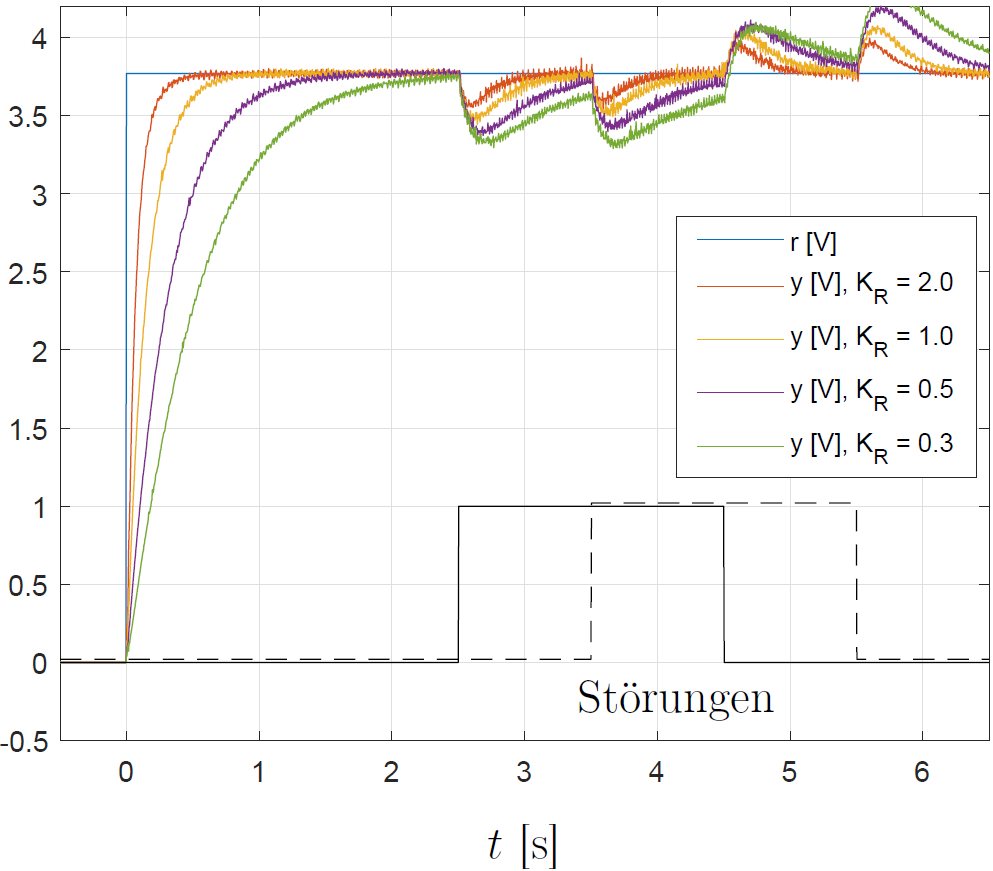
\includegraphics[width=\columnwidth]{images/gleichstromantrieb_pi-regler_step_response.png}
\end{minipage}


\subsection{Gleichstromantrieb mit PID / PD-Regler}{155}

\textbf{Der Regelkreis kann nicht weiter optimiert werden!} Der offenere Regelkreis entspricht bereits einem \textbf{Integrator},
was der \textbf{Idealfall} ist. 

Ein D-Anteil $\text{DT}_1$ wäre ungünstig, weil

\begin{itemize}
    \item Verstärkung von hohen Frequenzen \textrightarrow\ Erhöhung des Rauschens
    \item Verbesserung der Phasenreserve \textrightarrow\ unnötig bei $\Phi_{\rm RES} = 90 \degree$
\end{itemize}

Allenfalls sinnvoll wäre ein Tiefpassfilter für den P-Anteil ($\text{PT}_1$ statt P), um das Rauschen der Stellgrösse zu 
verkleinern \textrightarrow\ Reduktion der Phasenreserve!


\subsection{Gleichstromantrieb mit Totzeit mit PI-Regler}{157-159}

Das bisherige Modell der Strecke soll um eine Totzeit $T_t$ erweitert werden. Als Regler wird weiterhin ein PI-Regler eingesetzt.
Die Ergebnisse werden dadurch massiv schlechter!

$$ \text{UTF Stecke mit Totzeit} \quad G_S(s) = \frac{K_1}{s + 1} e^{-s T_t} $$
$$ \text{UTF Regelkreis} \quad G_0(s) = G_S(s) \cdot G_R(s) = \frac{K_1}{s + 1} e^{-s T_t} \cdot K_R \frac{1 + T_N s}{T_N s}
    \overset{T_N = T}{=} \frac{K_1 K_R}{s T} e^{-s T_t} $$

Die UTF des offenen Regelkreises $G_0(s)$ entspricht keinem Integrator mehr. Somit wird die UTF des geschossenen Regelkreises 
$G_f(s)$ keinem $\text{PT}_1$-System mehr entsprechen. 


\subsubsection{Effekte im Bode- und Nyquistdiagramm / Sprungantwort}

\begin{itemize}
    \item Amplitudengang unverändert, gleiche Durchtrittsfrequenz
    \item Phasengang wird schlechter (zusätzliche Phasenverzögerung), die $-180 \degree$ Phase wird bei tieferer
        Frequenz erreicht - die Verstärkungsreserve sinkt dadurch
    \item Die Phase bei der Durchtrittsfrequenz ist negativer, die Phasenreserve sinkt
\end{itemize}

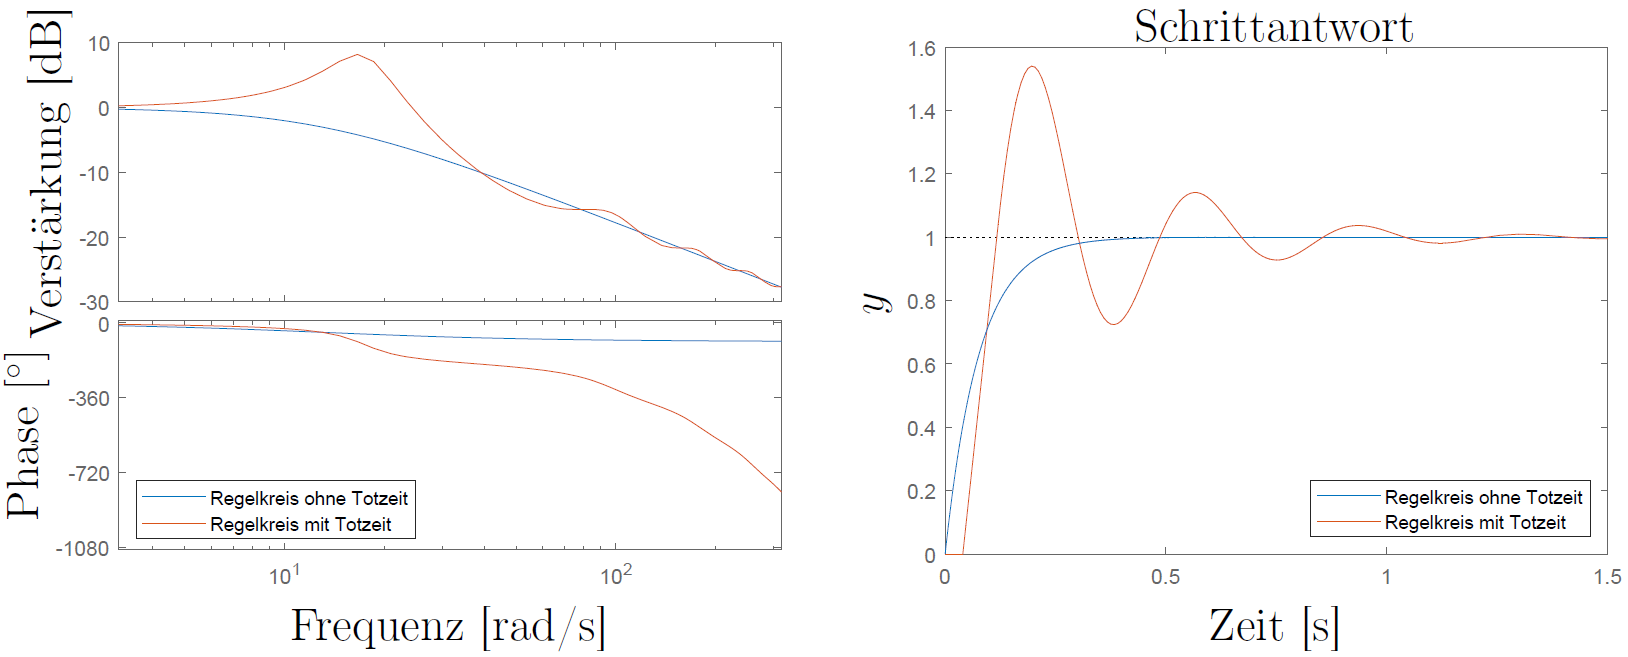
\includegraphics[width=\columnwidth]{images/gleichstromantrieb_pi-regler_totzeit_step_response.png}


\subsection{Gleichstromantrieb mit Totzeit mit PID-Regler}{160-162}

Um der Totzeit $T_t$ entgegnzuwirken, wird dem PI-Regler ein Lead-Glied (entspricht einem PD-Regler) in serie geschaltet 
\textrightarrow\ PID-Regler in multiplikativer Form (Abschnitt~\ref{PID-Regler multiplikative Form})

\medskip
Dies hat folgende Effekte:
\begin{outline}
    \1 Nyquistkurve wird bei der Durchtrittsfrequenz aktiv durch den Regler 'zurückgedreht' 
        \2 Effekt der Totzeit nicht für alle Frequenzen kompentireren, sondern in einem bestimmten Frequenzbereich
        \2 Im Bodediagramm: Phase bei $0 \, \deci \bel$ 
    \1 Serieschaltung eines Lead-Glieds (PD-Regler) zum PI-Regler \textrightarrow\ PID-Regler \\
        \textrightarrow\ Lead-Glied siehe Abschnitt ~\ref{Lead-Lag-Glied}
\end{outline}


\subsubsection{Auswirkungen des Lead-Glieds / PD-Reglers}

\begin{itemize}
    \item Phase und Verstärkung werden angehoben
    \item Zeitkonstante wird kleiner (Regler wird schneller)
\end{itemize}

\begin{minipage}[c]{0.4\columnwidth}
    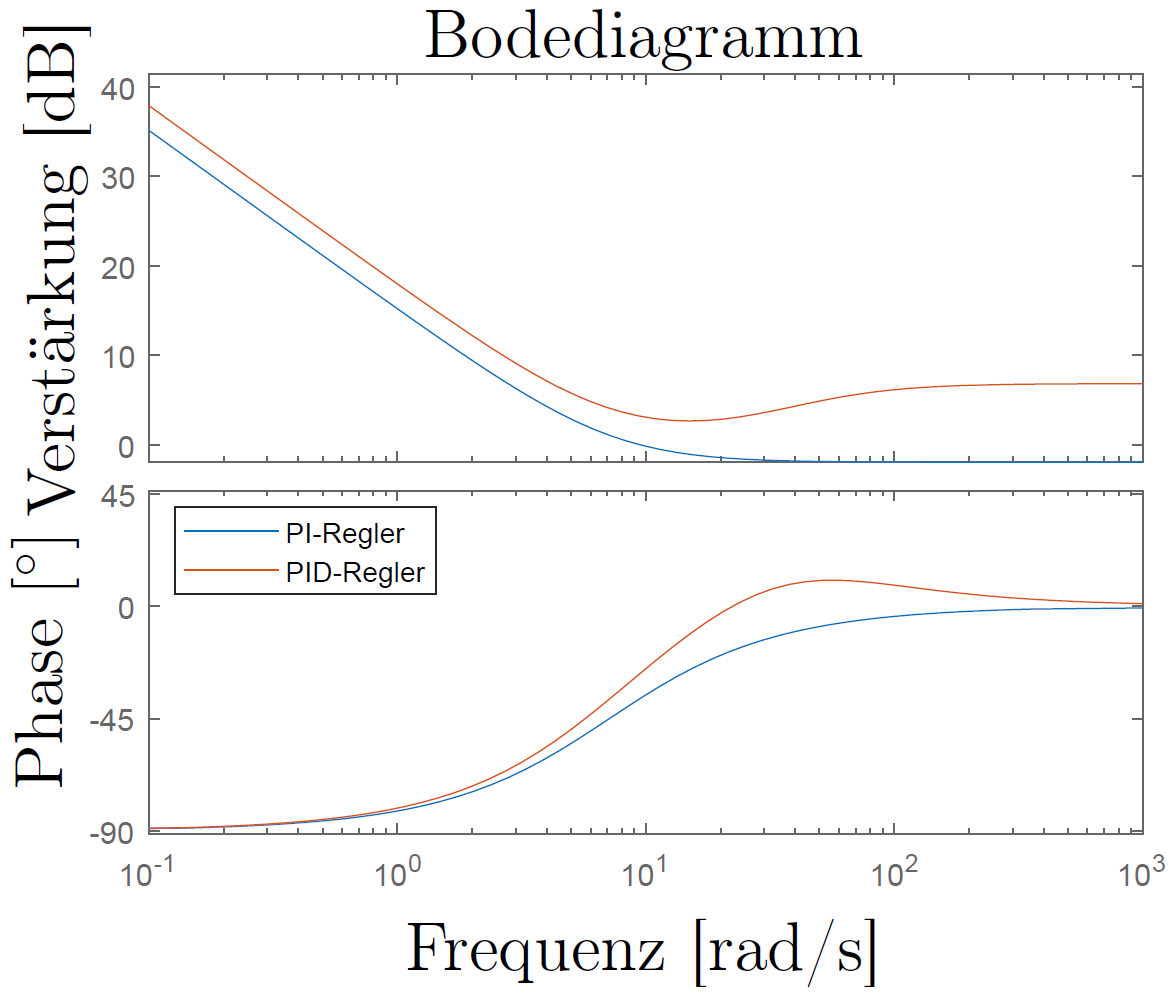
\includegraphics[width=\columnwidth]{images/gleichstromantrieb_pid-regler_bodediagramm.png}
\end{minipage}
\hfill
\begin{minipage}[c]{0.4\columnwidth}
    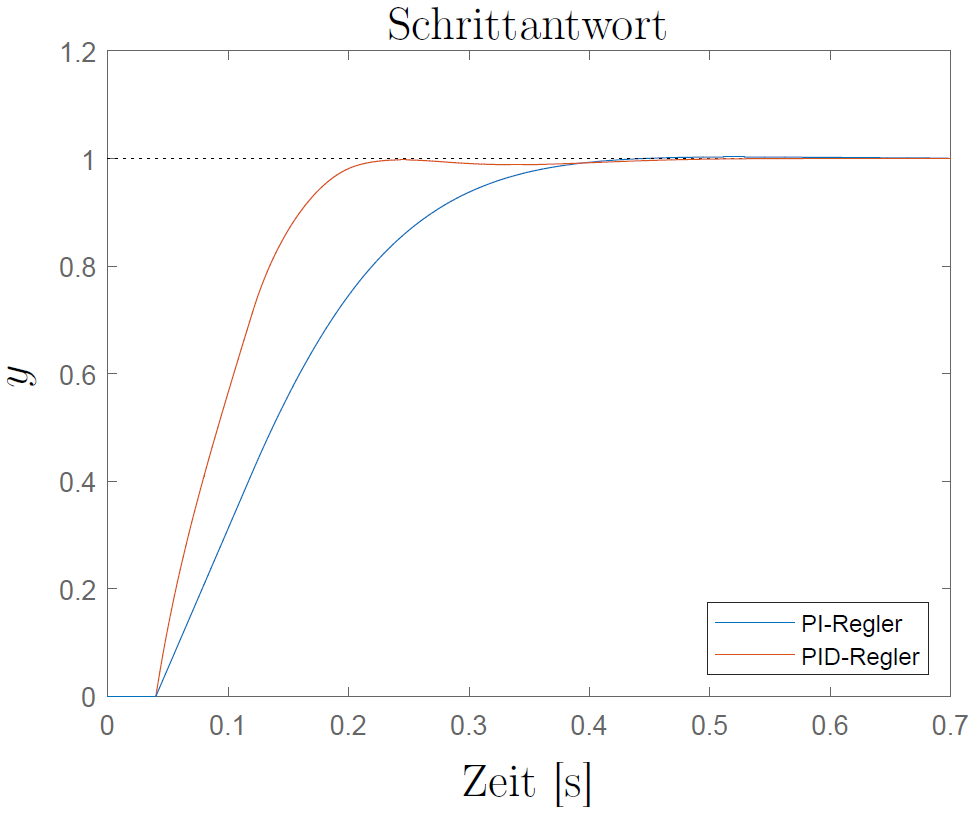
\includegraphics[width=\columnwidth]{images/gleichstromantrieb_pid-regler_step_response.png}
\end{minipage}

